\begin{center}
\begin{huge}
Διαδρομή Λαμία$\,\to\,$Αθήνα
\end{huge}
\addcontentsline{toc}{section}{Διαδρομή Λαμία προς Αθήνα}
\section*{Αποφυγή διοδίων Λαμίας\footnote{Λαμβάνοντας υπόψη την αναλογία ταλαιπωρίας/αξίας κομίστρου, επιλέγουμε να πληρώσουμε το κόμιστρο του συγκεκριμένου σταθμού. Στο συγκεκριμένο κομμάτι γίνονται έργα και ενδεχομένως κάποιοι δρόμοι να μην υφίστανται. Σε περίπτωση αλλαγών στο οδικό δίκτυο ή για τυχόν παραλείψεις δε φέρουμε ευθύνη.}}
\end{center}
\addcontentsline{toc}{subsection}{Αποφυγή διοδίων Λαμίας}
Ερχόμενοι από την Εθνική οδό Λαμίας - Λάρισας εισερχόμαστε στον Ε65 και συνεχίζουμε ευθεία μέχρι να φτάσουμε στη διχάλα της \textbf{εικόνας 26} όπου και κατευθυνόμαστε δεξιά.
 
\begin{figure}[H]
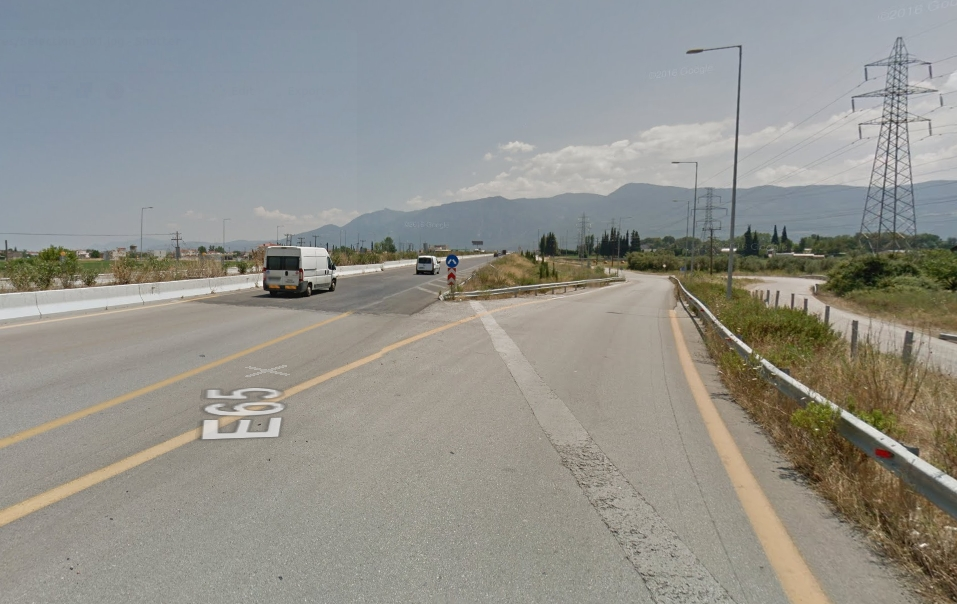
\includegraphics[width=\textwidth]{images/lamia-athina/lamia/lamia_002.jpg} 
\caption{Στρίβουμε δεξιά} 
\end{figure}

Μόλις φτάσουμε στη διασταύρωση της \textbf{εικόνας 27} (περίπου 200μ) περνάμε αριστερά και κάτω από το γεφυράκι και στη συνέχεια στρίβουμε δεξιά με κατεύθυνση προς Ανθήλη [\textbf{εικόνα 28}]. 
\begin{figure}[H]
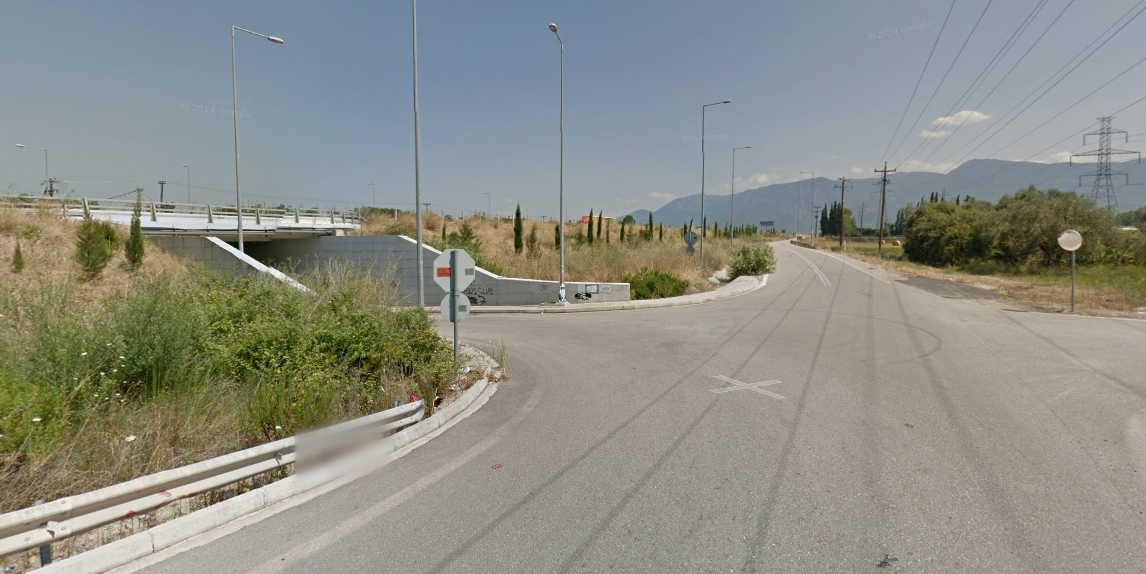
\includegraphics[width=\textwidth]{images/lamia-athina/lamia/lamia_003.jpg}
\caption{Στρίβουμε αριστερά κάτω από τη γέφυρα}
\end{figure}
\begin{figure}[H]  
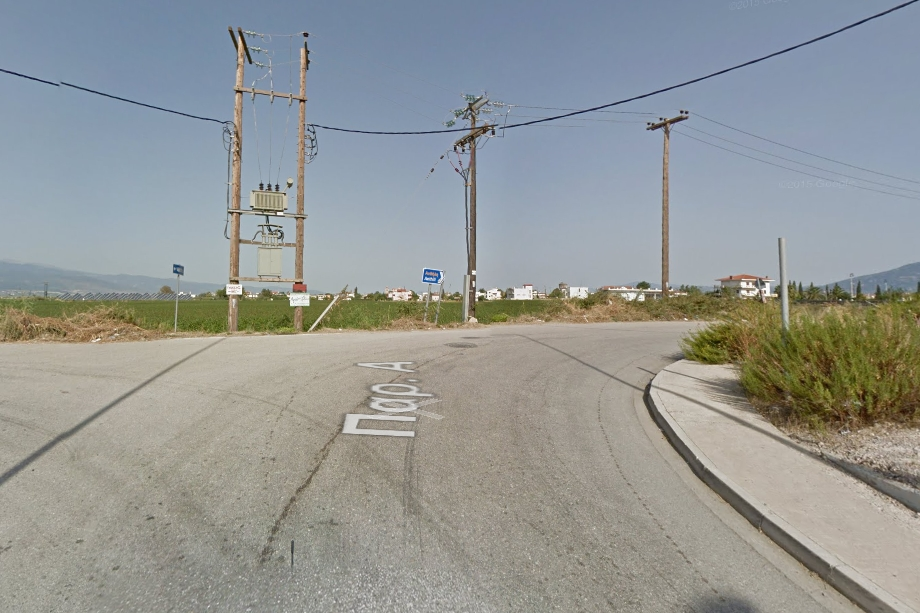
\includegraphics[width=\textwidth]{images/lamia-athina/lamia/lamia_004.jpg} 
\caption{Στρίβουμε δεξιά προς Ανθήλη} 
\end{figure}

Συνεχίζουμε για αρκετό κομμάτι του δρόμου ευθεία, περνάμε πίσω από τα Goodys και συνεχίζουμε μέχρι να φτάσουμε στο σημείο της \textbf{εικόνας 29} όπου και κάνουμε διαγώνια αριστερά. 
\begin{figure}[H]
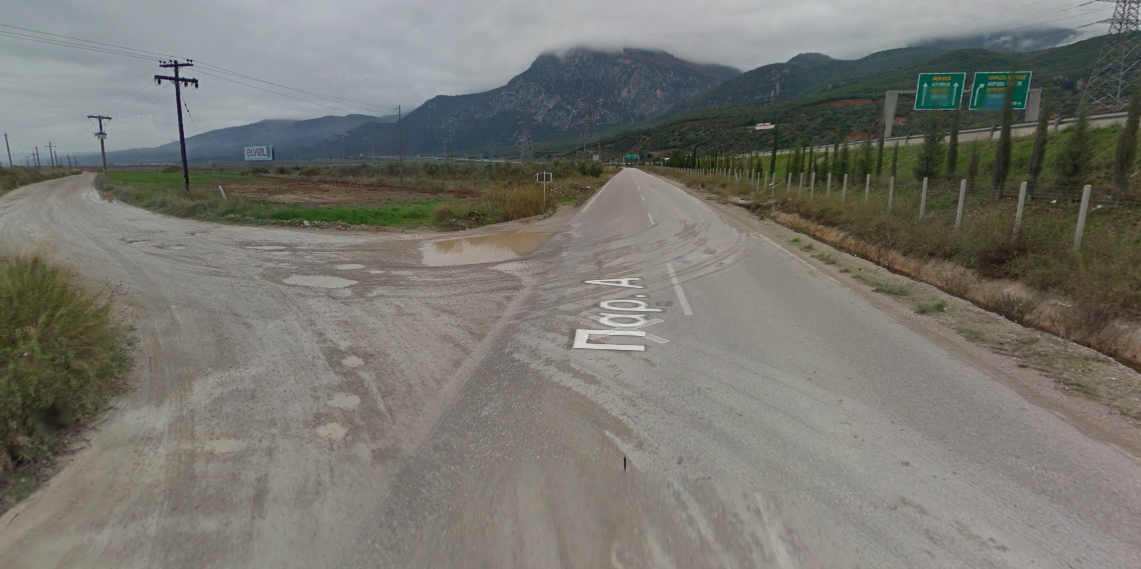
\includegraphics[width=\textwidth]{images/lamia-athina/lamia/lamia_005.jpg}
\caption{Στρίβουμε διαγώνια αριστερά} 
\end{figure}

Συνεχίζουμε με κατεύθυνση προς Θερμοπύλες. Μόλις μπούμε στις Θερμοπύλες συνεχίζουμε ευθεία κάτω από τη γέφυρα και αμέσως δεξιά και στην πρώτη έξοδο δεξιά για να μπούμε στην Επαρχιακή οδό Αταλάντης-Εξάρχου. Συνεχίζουμε ευθεία μέχρι να βρεθούμε στον κυκλικό κόμβο των Καμμένων Βούρλων [\textbf{εικόνα 30}] και στη 2η έξοδο κατευθυνόμαστε δεξιά κάτω από τη γέφυρα και αμέσως αριστερά όπου και θα βρεθούμε στην ΠΕΟ (Παλιά Εθνική Οδό).
\begin{figure}[H]
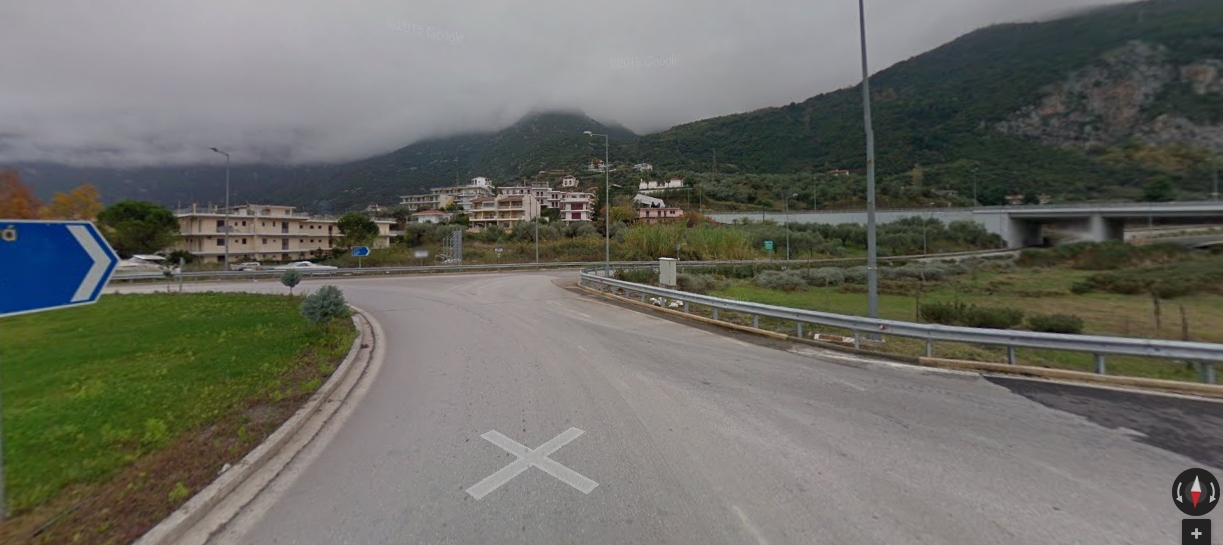
\includegraphics[width=\textwidth]{images/lamia-athina/lamia/lamia_006.jpg}
\caption{Στρίβουμε δεξιά περνάμε κάτω από τη γέφυρα και αμέσως αριστερά}  
\end{figure}

Προχωρούμε ευθεία μέχρι το σημείο της διασταύρωσης της \textbf{εικόνας 31} (είναι το ίδιο που χρησιμοποιούμε και για κατεύθυνση προς Λαμία) όπου κάνουμε δεξιά και προχωρούμε περνώντας κάτω από τη γέφυρα. 
\begin{figure}[H]
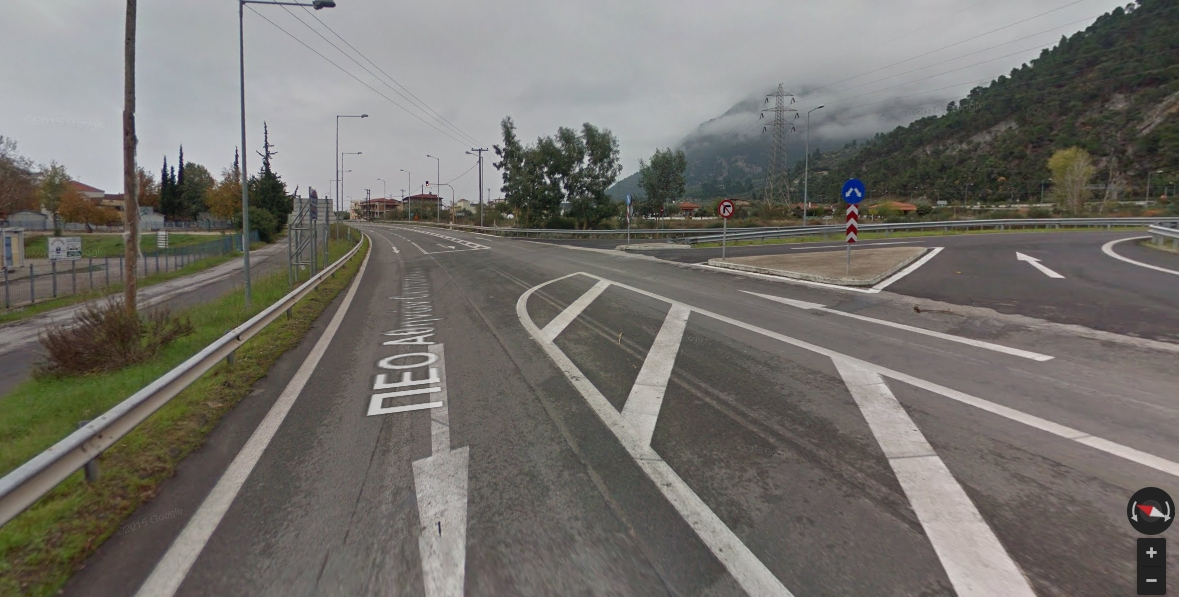
\includegraphics[width=\textwidth]{images/lamia-athina/lamia/lamia_007.jpg}
\caption{Στρίβουμε δεξιά} 
\end{figure}


Βγαίνουμε στην Εθνική Οδό.

\newpage
\begin{center}
\section*{Αποφυγή διοδίων Τραγάνας}
\end{center}
\addcontentsline{toc}{subsection}{Αποφυγή διοδίων Τραγάνας}
Βρισκόμαστε στην ΕΟ. Αναζητούμε την ταμπέλα για Δελφούς-Αταλάντη \textbf{εικόνα 32} και στρίβουμε δεξιά. Στη διασταύρωση δεξιά [\textbf{εικόνα 33}] και αμέσως αριστερά [\textbf{εικόνα 34}]
\begin{figure}[H]
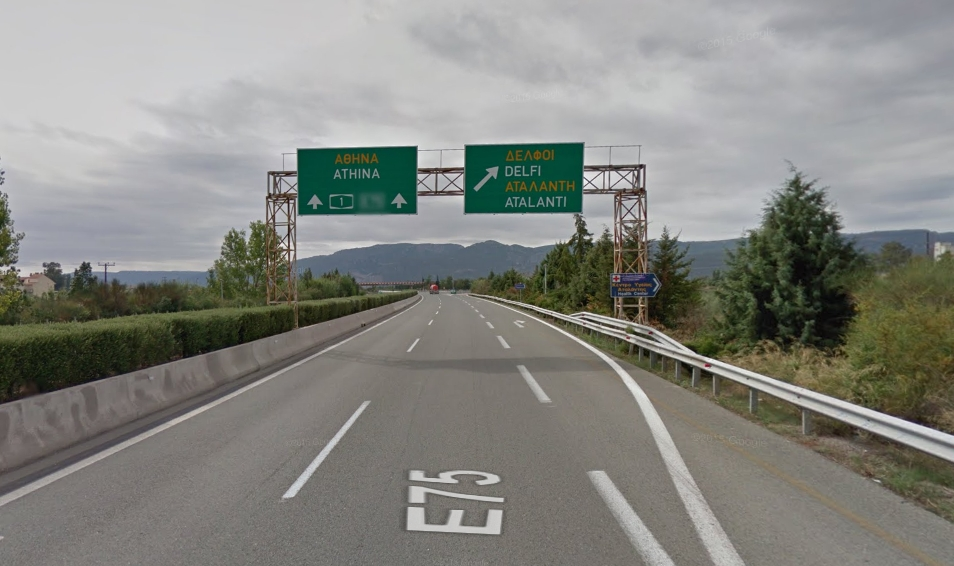
\includegraphics[width=\textwidth]{images/lamia-athina/tragana/tragana_008.jpg}
\caption{Στρίβουμε δεξιά}
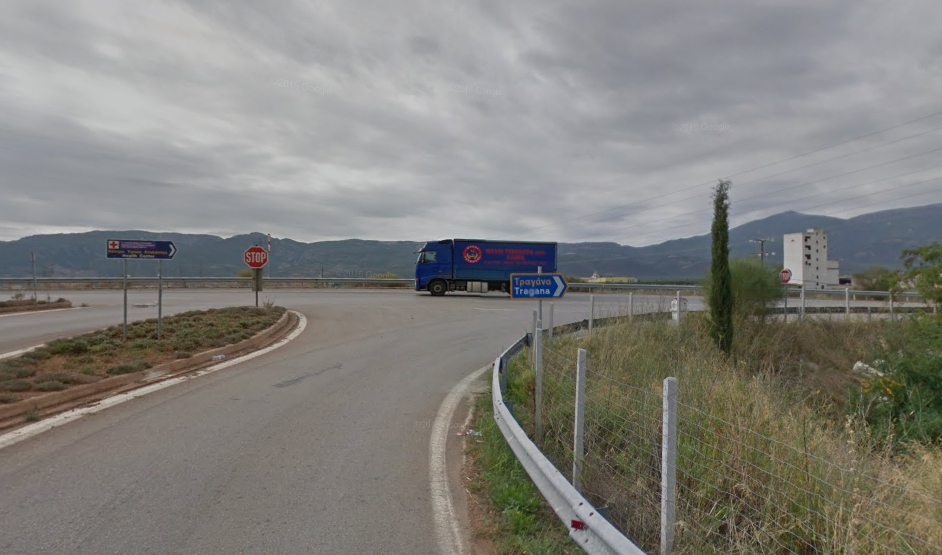
\includegraphics[width=\textwidth]{images/lamia-athina/tragana/tragana_009.jpg} 
\caption{Στρίβουμε δεξιά...}
\end{figure}
\begin{figure}[H]
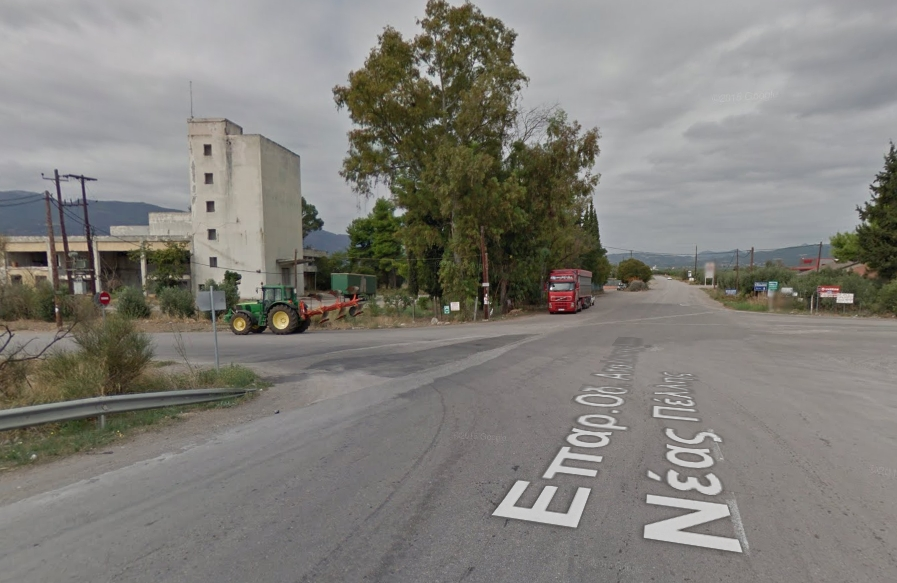
\includegraphics[width=\textwidth]{images/lamia-athina/tragana/tragana_010.jpg} 
\caption{...και αμέσως αριστερά}
\end{figure}
Συνεχίζουμε ευθεία μέχρι να περάσουμε στα αριστερά μας τα διόδια της Τραγάνας. Στο τέλος του δρόμου πηγαίνουμε δεξιά (ταμπέλα με κατεύθυνση Προσκυνά) [\textbf{εικόνα 35}]
\begin{figure}[H]
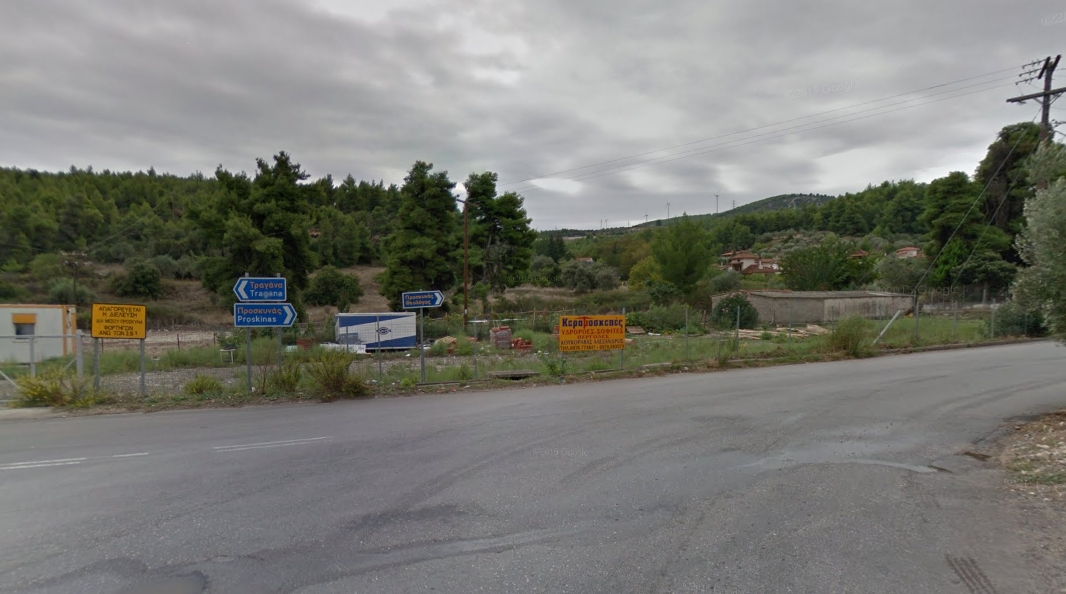
\includegraphics[width=\textwidth]{images/lamia-athina/tragana/tragana_011.jpg} 
\caption{στρίβουμε δεξιά}
\end{figure}
Μέσα στο χωριό στη διχάλα συνεχίζουμε αριστερά [\textbf{εικόνα 36}] (Ταμπέλα προς Εθνική Οδό)
\begin{figure}[H]
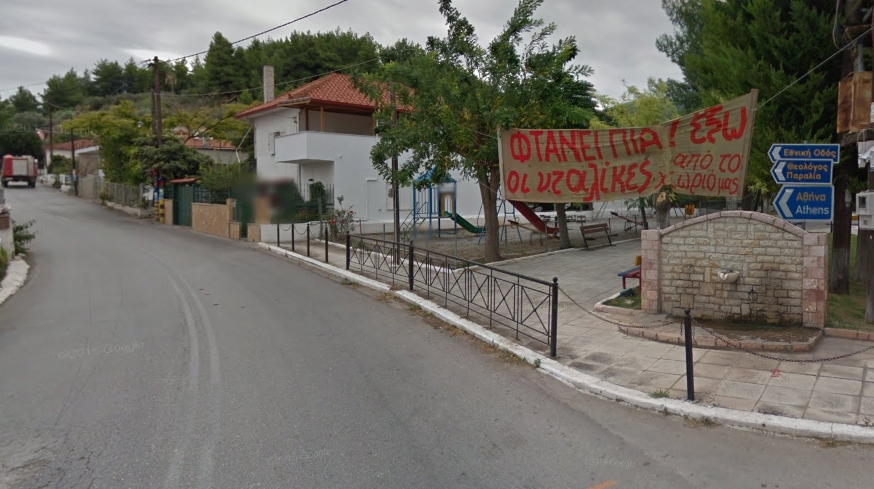
\includegraphics[width=\textwidth]{images/lamia-athina/tragana/tragana_012.jpg} 
\caption{στρίβουμε αριστερά}
\end{figure}
Συνεχίζουμε ευθεία μέχρι τη διασταύρωση όπου κάνουμε δεξιά προς ΕΟ [\textbf{εικόνα 37}]
\begin{figure}[H]
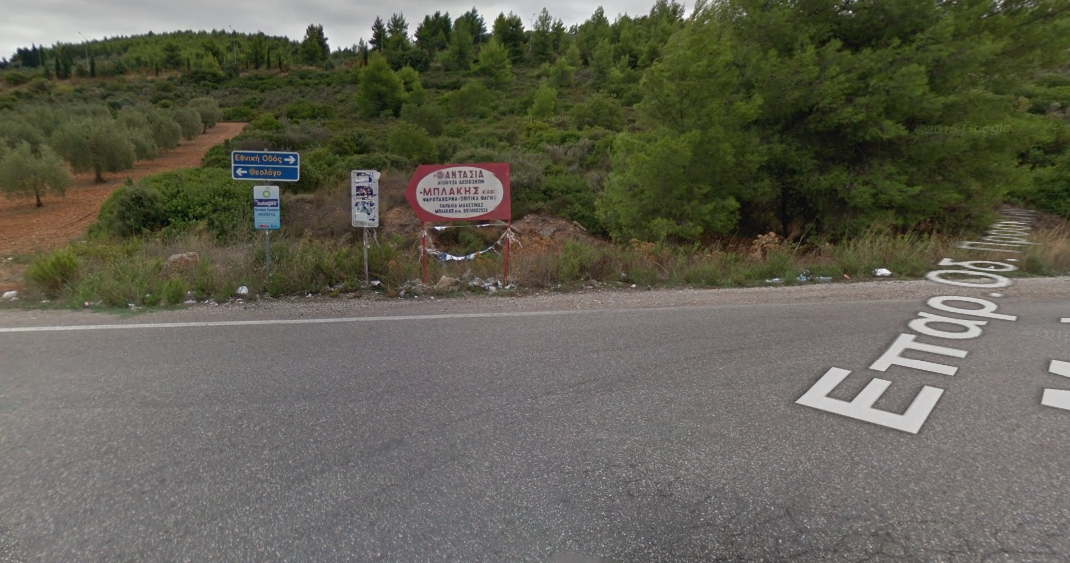
\includegraphics[width=\textwidth]{images/lamia-athina/tragana/tragana_013.jpg} 
\caption{στρίβουμε δεξιά}
\end{figure}
Τέλος φτάνουμε στη διασταύρωση [\textbf{εικόνα 38}]που βρίσκεται αμέσως μετά το βενζινάδικο της Elin. Εκεί συνεχίζουμε ευθεία απέναντι.
\begin{figure}[H]
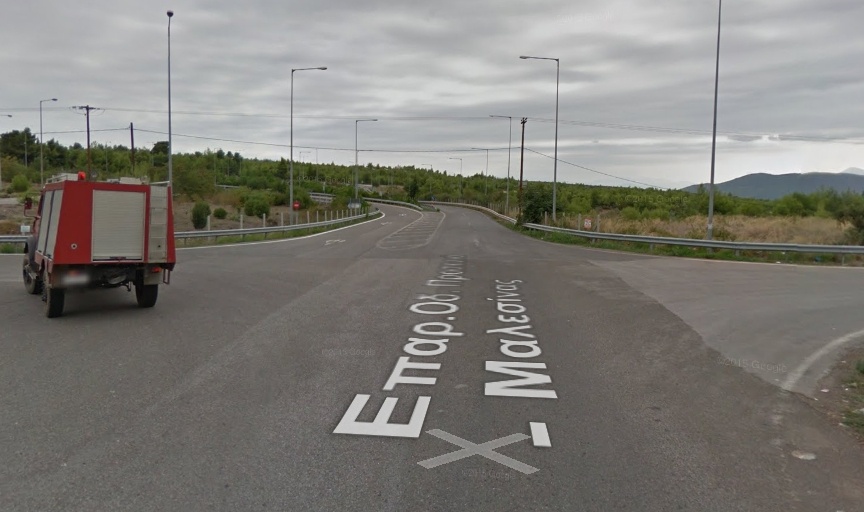
\includegraphics[width=\textwidth]{images/lamia-athina/tragana/tragana_014.jpg} 
\caption{κατευθυνόμαστε ευθεία απέναντι}
\end{figure}
Βγαίνουμε στην Εθνική Οδό.
\newpage
\begin{center}
\section*{Αποφυγή διοδίων Θήβας}
\end{center}
\addcontentsline{toc}{subsection}{Αποφυγή διοδίων Θήβας}
Μπαίνουμε στο καφέ 90 και εισερχόμαστε στον παράδρομο που πάει ακριβώς παράλληλα με την ΕΟ. Περνάμε στο αριστερό μας χέρι τα διόδια της Θήβας και στη διασταύρωση κάνουμε αριστερά και ανεβαίνουμε στη γέφυρα [\textbf{εικόνα 39}]. 
\begin{figure}[H]
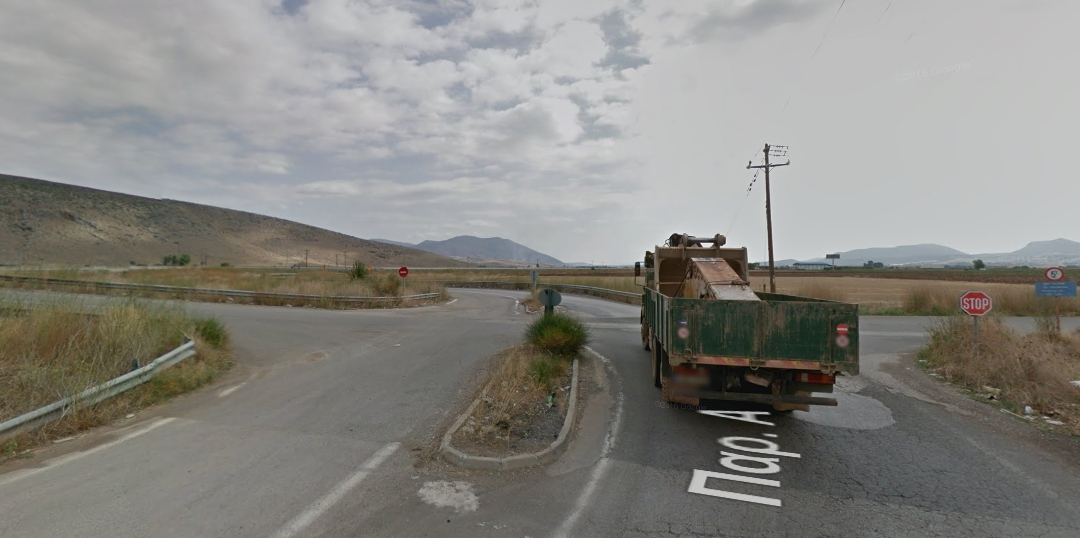
\includegraphics[width=\textwidth]{images/lamia-athina/thiva/thiva_015.jpg} 
\caption{στρίβουμε αριστερά πάνω στη γέφυρα}
\end{figure}
Αφότου περάσουμε απέναντι θα μας βγάλει στη διασταύρωση όπου δεξιά μας είναι το 90 (το απέναντι 90 από αυτό που μπήκαμε). Στρίβουμε αριστερά και συνεχίζουμε ευθεία. Θα περάσουμε 2 διασταυρώσεις όπου και στις 2 θα περάσουμε απέναντι [\textbf{εικόνες 40 - 41}].
\begin{figure}[H]
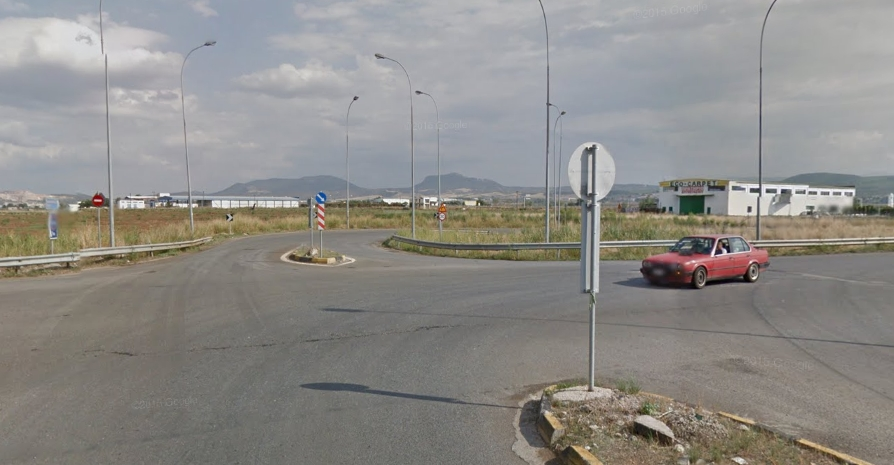
\includegraphics[width=\textwidth]{images/lamia-athina/thiva/thiva_016.jpg} 
\caption{συνεχίζουμε ευθεία απέναντι}
\end{figure}
\begin{figure}[H]
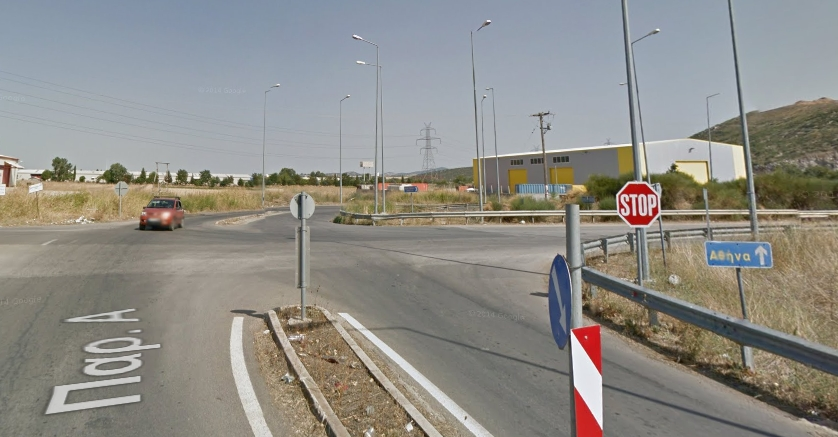
\includegraphics[width=\textwidth]{images/lamia-athina/thiva/thiva_017.jpg} 
\caption{συνεχίζουμε ευθεία απέναντι (Ταμπέλα προς Αθήνα)}
\end{figure}
Στο τέλος του δρόμου στη διασταύρωση στρίβουμε δεξιά προς Αθήνα [\textbf{εικόνα 42}]
\begin{figure}[H]
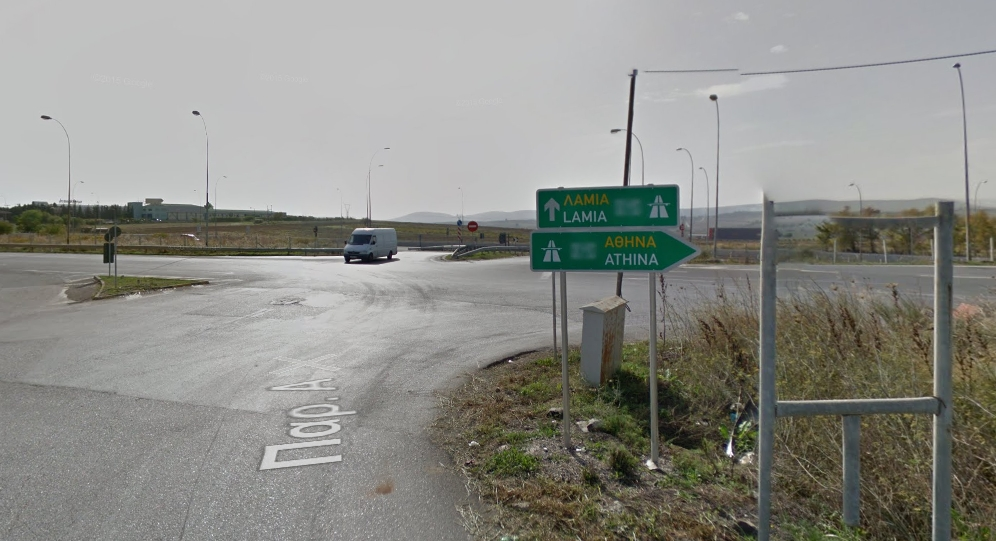
\includegraphics[width=\textwidth]{images/lamia-athina/thiva/thiva_018.jpg} 
\caption{στρίβουμε δεξιά}
\end{figure}
Περνάμε πάνω από τη γέφυρα και αμέσως παίρνουμε την έξοδο δεξιά όπως το βυτίο στην \textbf{εικόνα 43}
\begin{figure}[H]
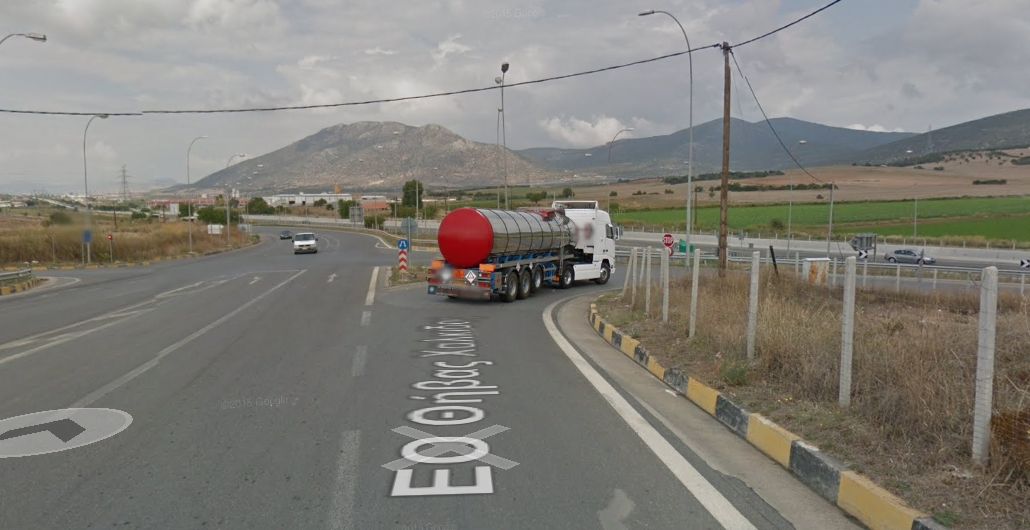
\includegraphics[width=\textwidth]{images/lamia-athina/thiva/thiva_019.jpg} 
\caption{στρίβουμε δεξιά}
\end{figure}
Βγαίνουμε στην Εθνική Οδό
\newpage
\begin{center}
\section*{Αποφυγή διοδίων Αφιδνών}
\end{center}
\addcontentsline{toc}{subsection}{Αποφυγή διοδίων Αφιδνών}
Βρισκόμαστε στην Εθνική οδό. Αναζητούμε την έξοδο προς Οινόη και κάνουμε δεξιά [\textbf{εικόνα 44}]
\begin{figure}[H]
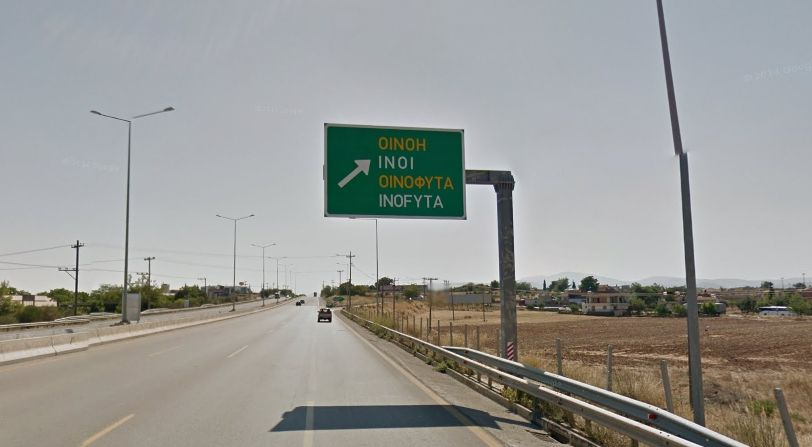
\includegraphics[width=\textwidth]{images/lamia-athina/afidnon/afidnon_020.jpg} 
\caption{στρίβουμε δεξιά}
\end{figure}
Αμέσως μετά στη διασταύρωση κάνουμε αριστερά [\textbf{εικόνα 45}]
\begin{figure}[H]
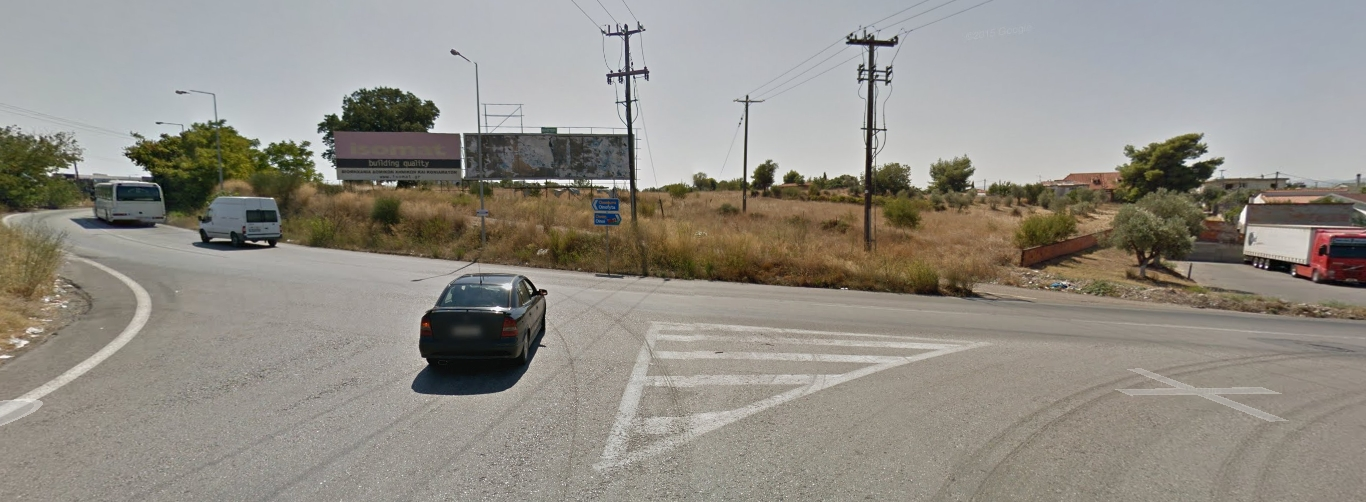
\includegraphics[width=\textwidth]{images/lamia-athina/afidnon/afidnon_021.jpg} 
\caption{στρίβουμε αριστερά}
\end{figure}
Συνεχίζουμε για ένα μεγάλο κομμάτι του δρόμου παράλληλα με την ΕΟ μέχρι να φτάσουμε στη διασταύρωση της εικόνας (είναι η πρώτη μεγάλη διασταύρωση που συναντάμε) όπου κάνουμε αριστερά [\textbf{εικόνα 46}] και αμέσως μετά μόλις περάσουμε κάτω από τη γέφυρα δεξιά [\textbf{εικόνα 47}].
\begin{figure}[H]
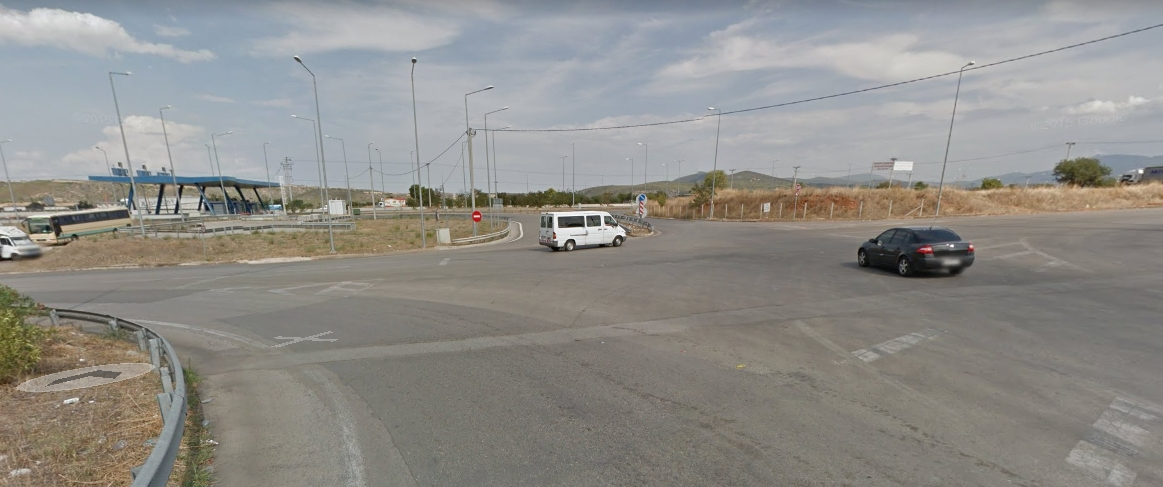
\includegraphics[width=\textwidth]{images/lamia-athina/afidnon/afidnon_022.jpg} 
\caption{στρίβουμε αριστερά...}
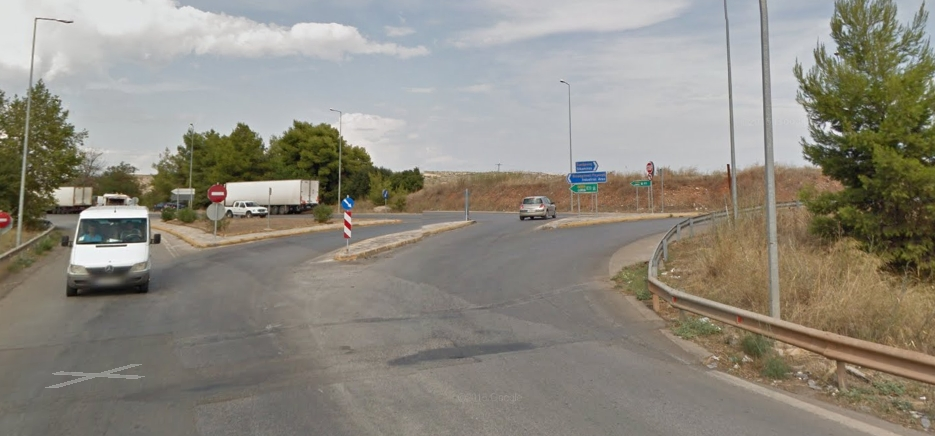
\includegraphics[width=\textwidth]{images/lamia-athina/afidnon/afidnon_023.jpg} 
\caption{... και αμέσως στρίβουμε δεξιά}
\end{figure}
Τώρα βρισκόμαστε στην ΠΕΟ Αθηνών Θεσσαλονίκης και συνεχίζουμε ευθεία μέχρι τη Μαλακάσα όπου και πάλι θα συνεχίσουμε ευθεία απέναντι όπως φαίνεται στην \textbf{εικόνα 48}.
\begin{figure}[H]
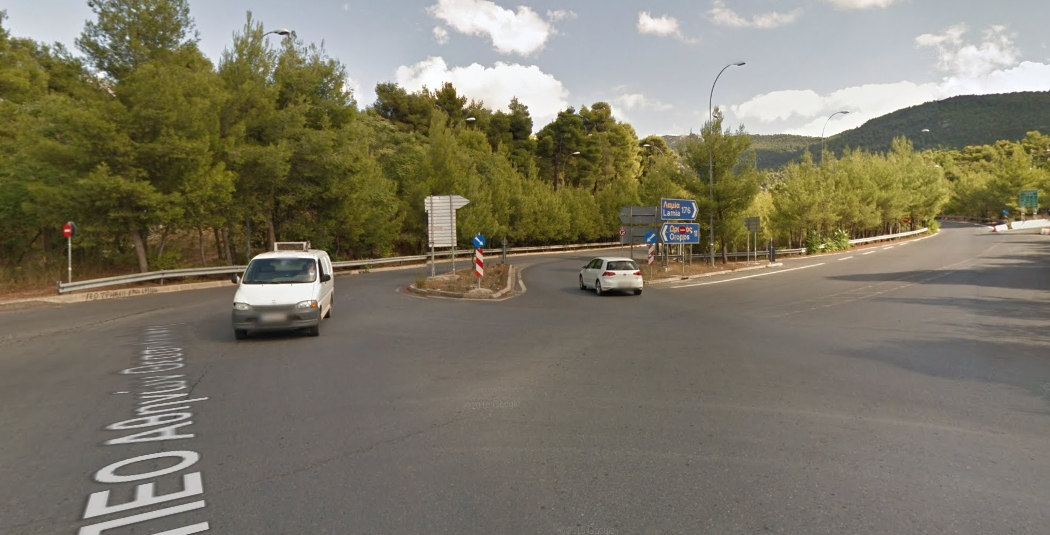
\includegraphics[width=\textwidth]{images/lamia-athina/afidnon/afidnon_024.jpg} 
\caption{συνεχίζουμε ευθεία απέναντι}
\end{figure}
Στην πορεία μας θα συναντήσουμε ακόμη μια διασταύρωση όπου και εκεί θα συνεχίσουμε απέναντι [\textbf{εικόνα 49}].
\begin{figure}[H]
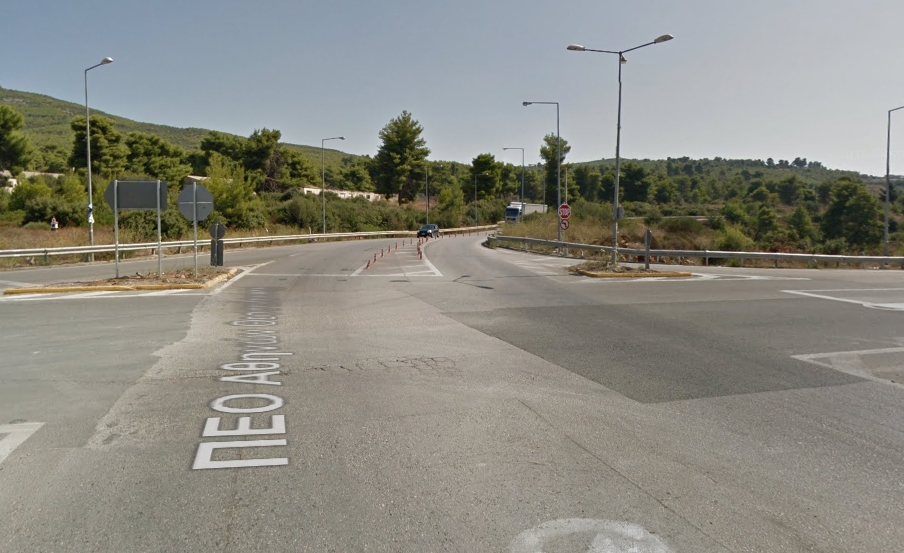
\includegraphics[width=\textwidth]{images/lamia-athina/afidnon/afidnon_025.jpg} 
\caption{συνεχίζουμε ευθεία απέναντι}
\end{figure}
Το επόμενο σημείο προσοχής είναι τα ανθοπωλεία που τα συναντάμε όπως φαίνεται και στην εικόνα από τη διακριτική ταμπέλα "ΦΥΤΑ". Στρίβουμε δεξιά [\textbf{εικόνα 50}].
\begin{figure}[H]
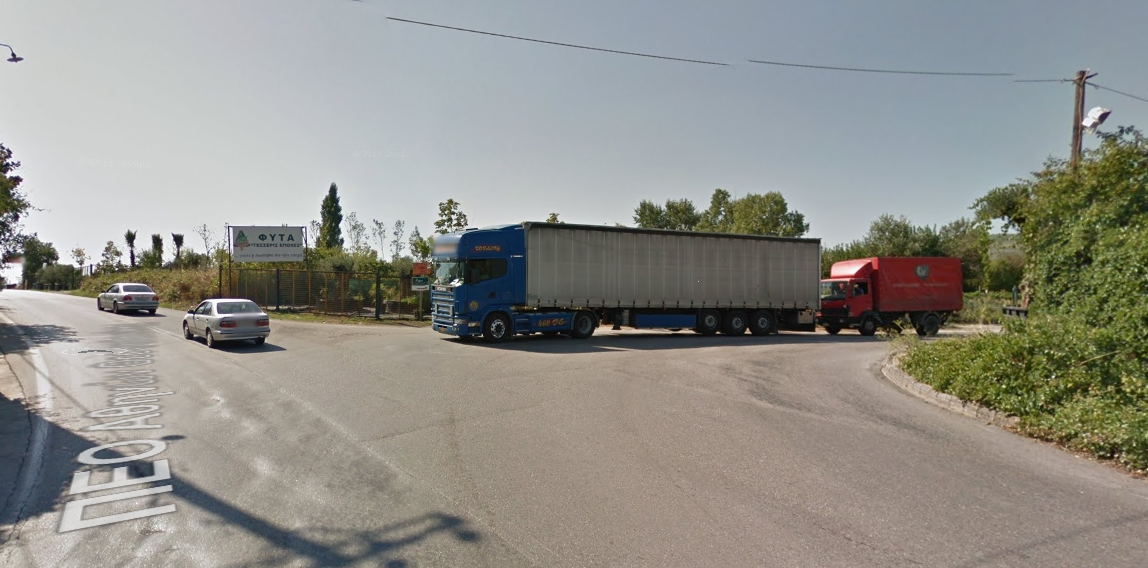
\includegraphics[width=\textwidth]{images/lamia-athina/afidnon/afidnon_026.jpg} 
\caption{στρίβουμε δεξιά}
\end{figure}
Στην πορεία περνάμε τα διόδια των Αφιδνών στο δεξί μας χέρι. Συνεχίζουμε ευθεία μέχρι να φτάσουμε στον κόμβο του Αγ.Στέφανου όπου στο φανάρι κάνουμε δεξιά [\textbf{εικόνα 51}].
\begin{figure}[H]
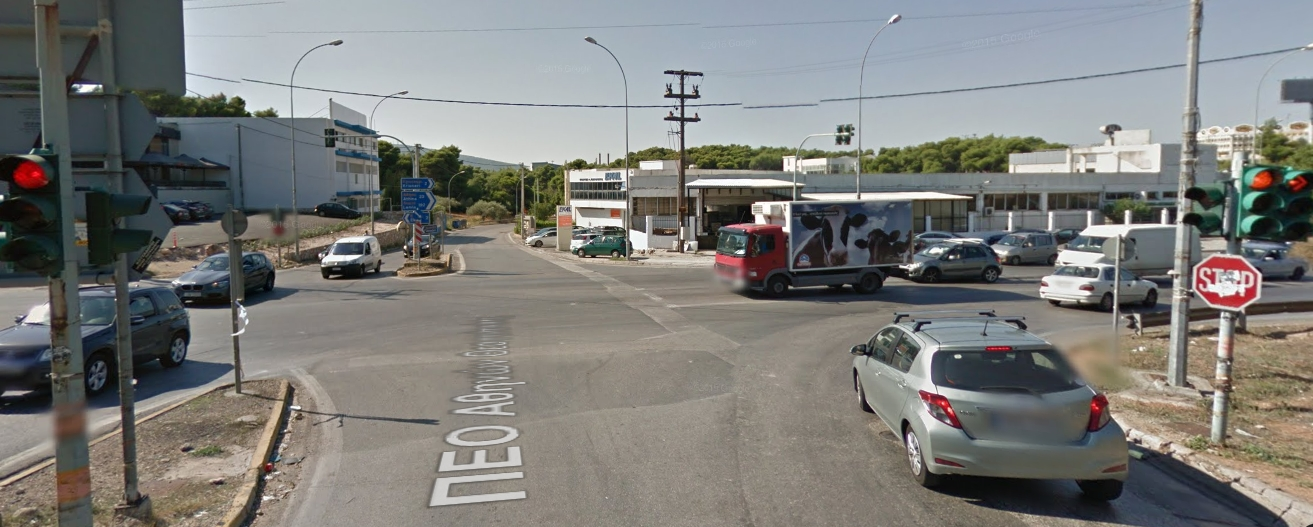
\includegraphics[width=\textwidth]{images/lamia-athina/afidnon/afidnon_027.jpg} 
\caption{στρίβουμε δεξιά}
\end{figure}
Περνάμε κάτω από τη γέφυρα και αμέσως στρίβουμε δεξιά [\textbf{εικόνα 52}]. Στη μικρή διχάλα που ακολουθεί πάμε αριστερά.
\begin{figure}[H]
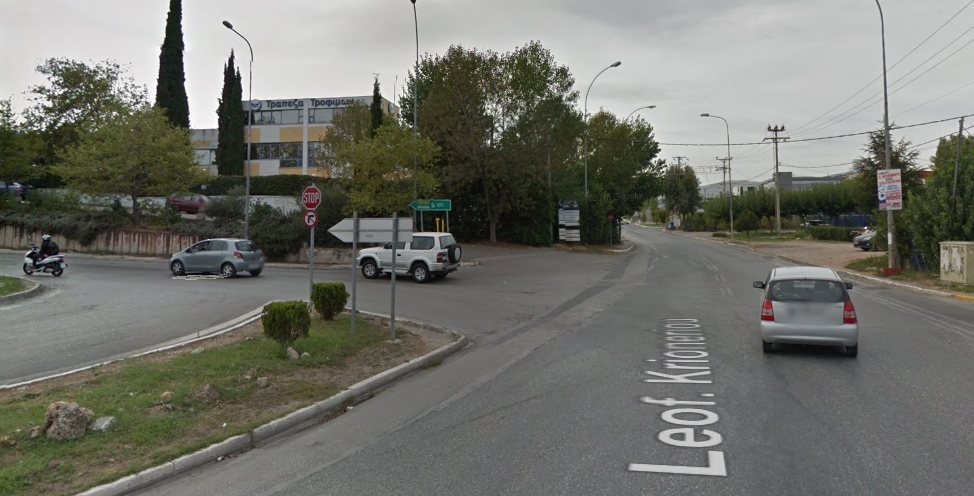
\includegraphics[width=\textwidth]{images/lamia-athina/afidnon/afidnon_028.jpg} 
\caption{στρίβουμε δεξιά}
\end{figure}
Βγαίνουμε στην Εθνική Οδό
\vspace{12pt}
\paragraph{Μέχρι την Αθήνα εξοικονομήσαμε}
\begin{itemize}
\item Αυτοκίνητο = 12.60€
\item Μηχανή = 8.75€
\item Φορτηγό ή μικρό ρυμουλκούμενο = 31.55€
\item Νταλίκα = 44.2€
\end{itemize}